\section{Introdução}
\begin{frame}{Definição do problema}

     \begin{figure}[ht]
            \begin{minipage}[b]{0.45\linewidth}
                \centering
                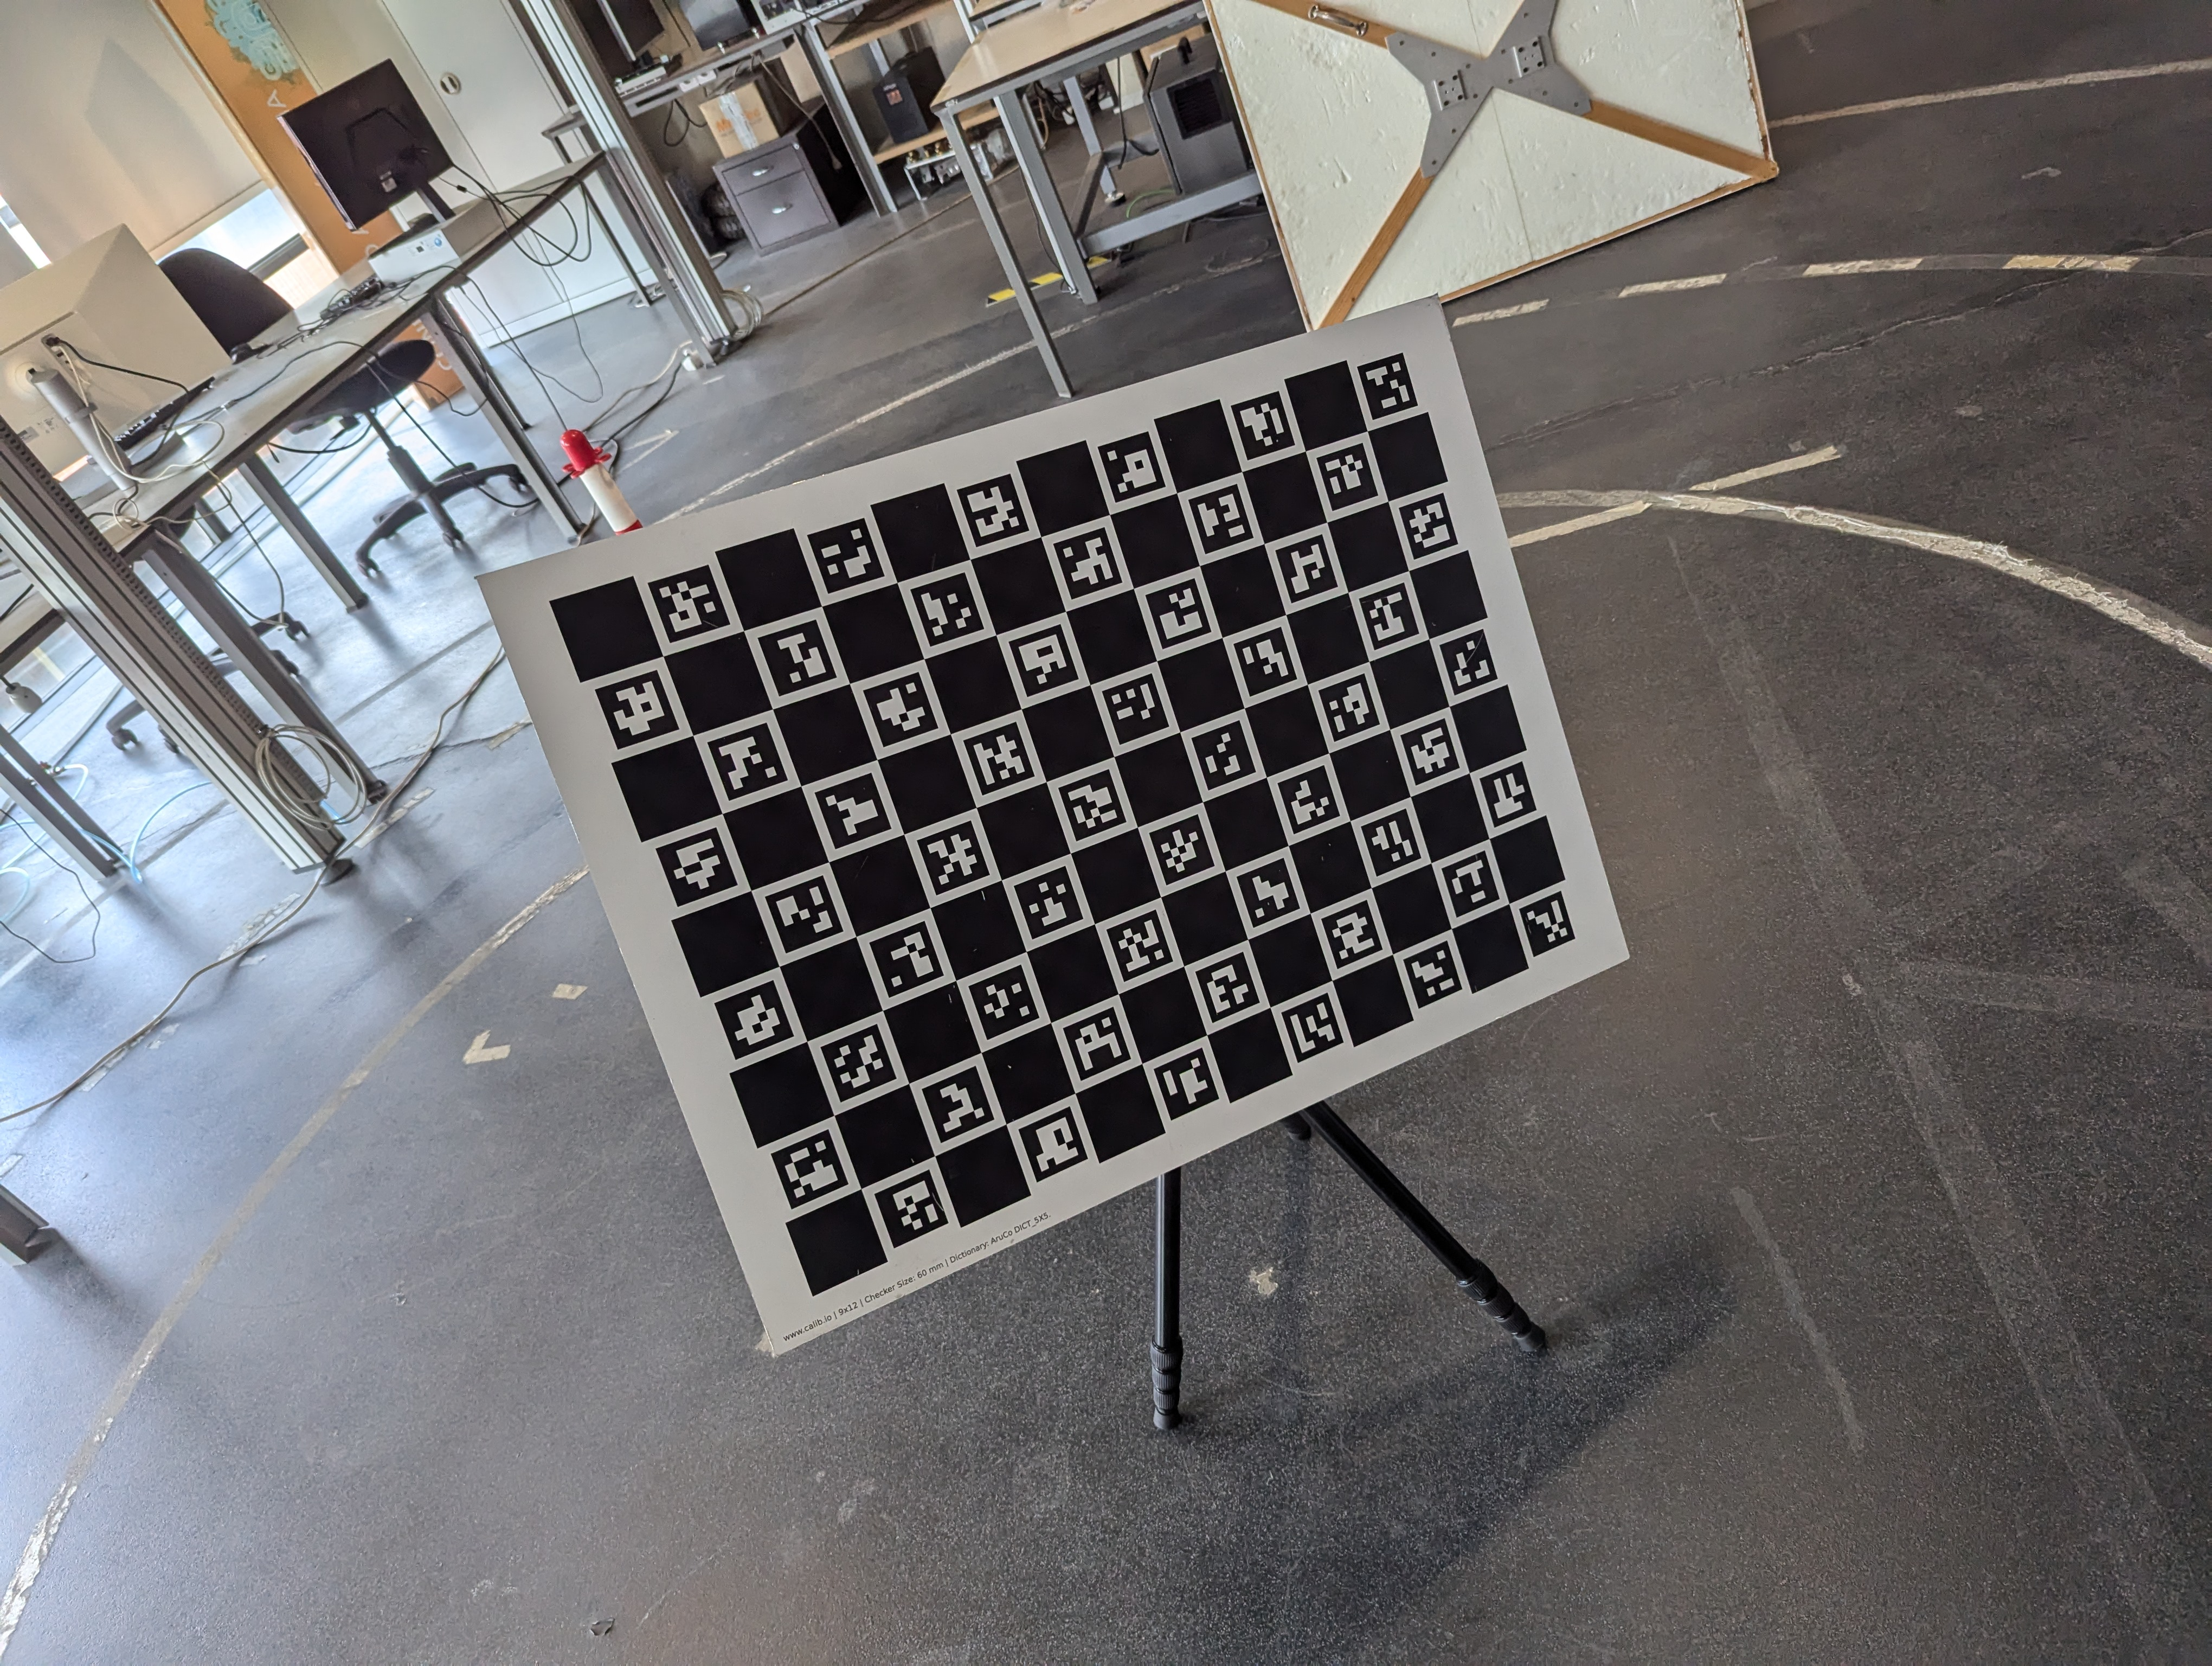
\includegraphics[width=1\textwidth]{resources/images/pattern_28.jpg}
                \captionsetup{labelformat=empty}
                \caption{Input image}
            \end{minipage}
            \hspace{0.5cm}
            \begin{minipage}[b]{0.45\linewidth}
                \centering
                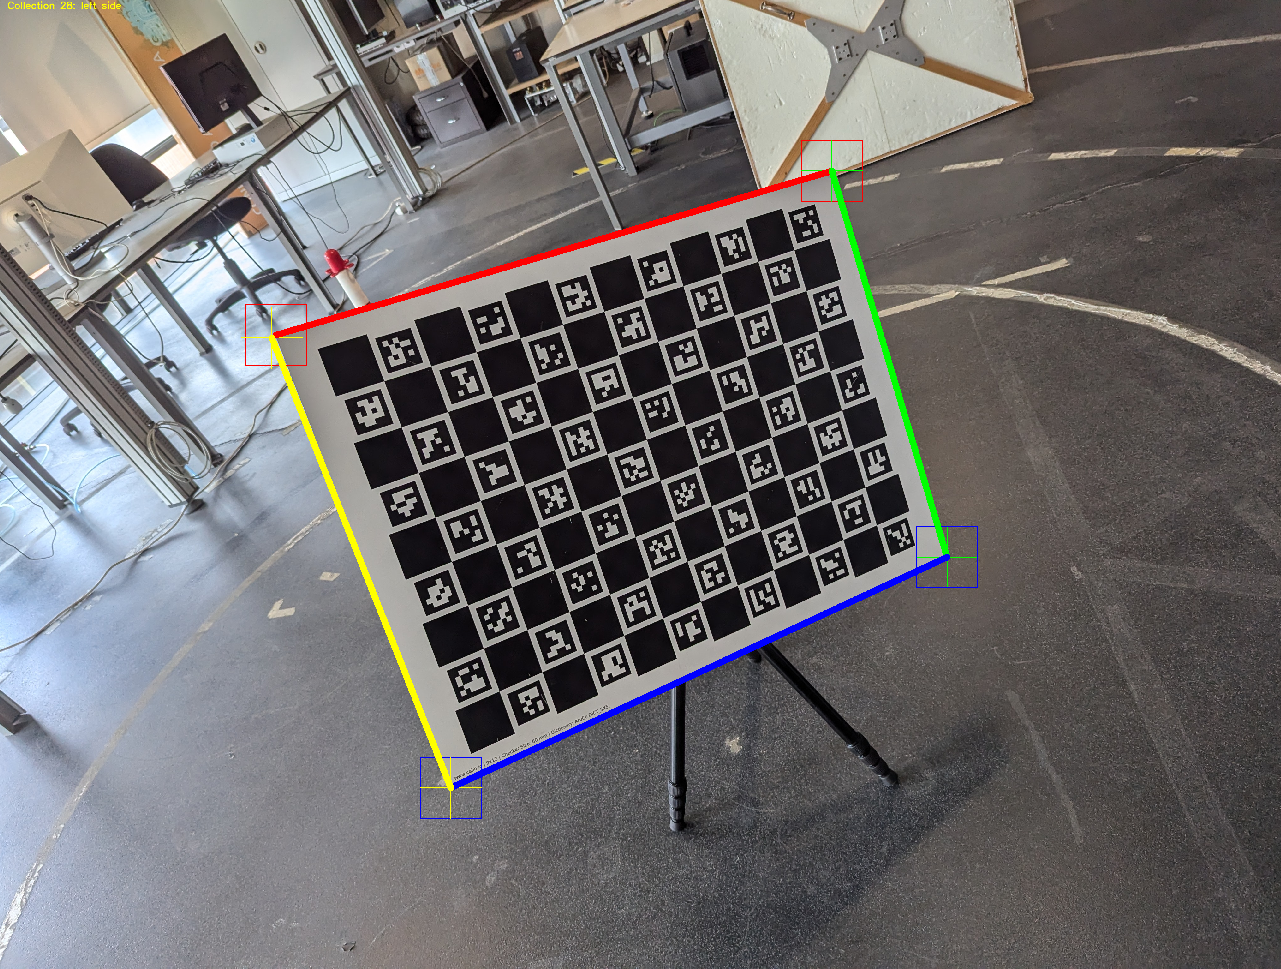
\includegraphics[width=1\textwidth]{resources/images/pattern_28_lines.png}
                \captionsetup{labelformat=empty}
                \caption{Desired Output Image}
            \end{minipage}
        \end{figure}
    
\end{frame}

\begin{frame}[c]{Escolha do tipo de rede}{Modelos de Segmentação}

  \begin{center}
    \begin{minipage}{0.7\textwidth}
      \begin{itemize}
      \Large
      \item<1-> Número de cantos variável visíveis na imagem;
      \item<1-> Possíveis obstruções parciais do padrão;
      \item<2-> Solução CNN + FC inviável por tamanho do output variavél;
      \item<3-> Rede de segmentação evita todos os possíveis os edge cases.
      \end{itemize}
    \end{minipage}
  \end{center}

    
  \end{frame}


\begin{frame}{Tipos de redes de segmentação}

    \begin{columns}

      \column{0.4\textwidth}
        \begin{figure}[h]
            \centering
            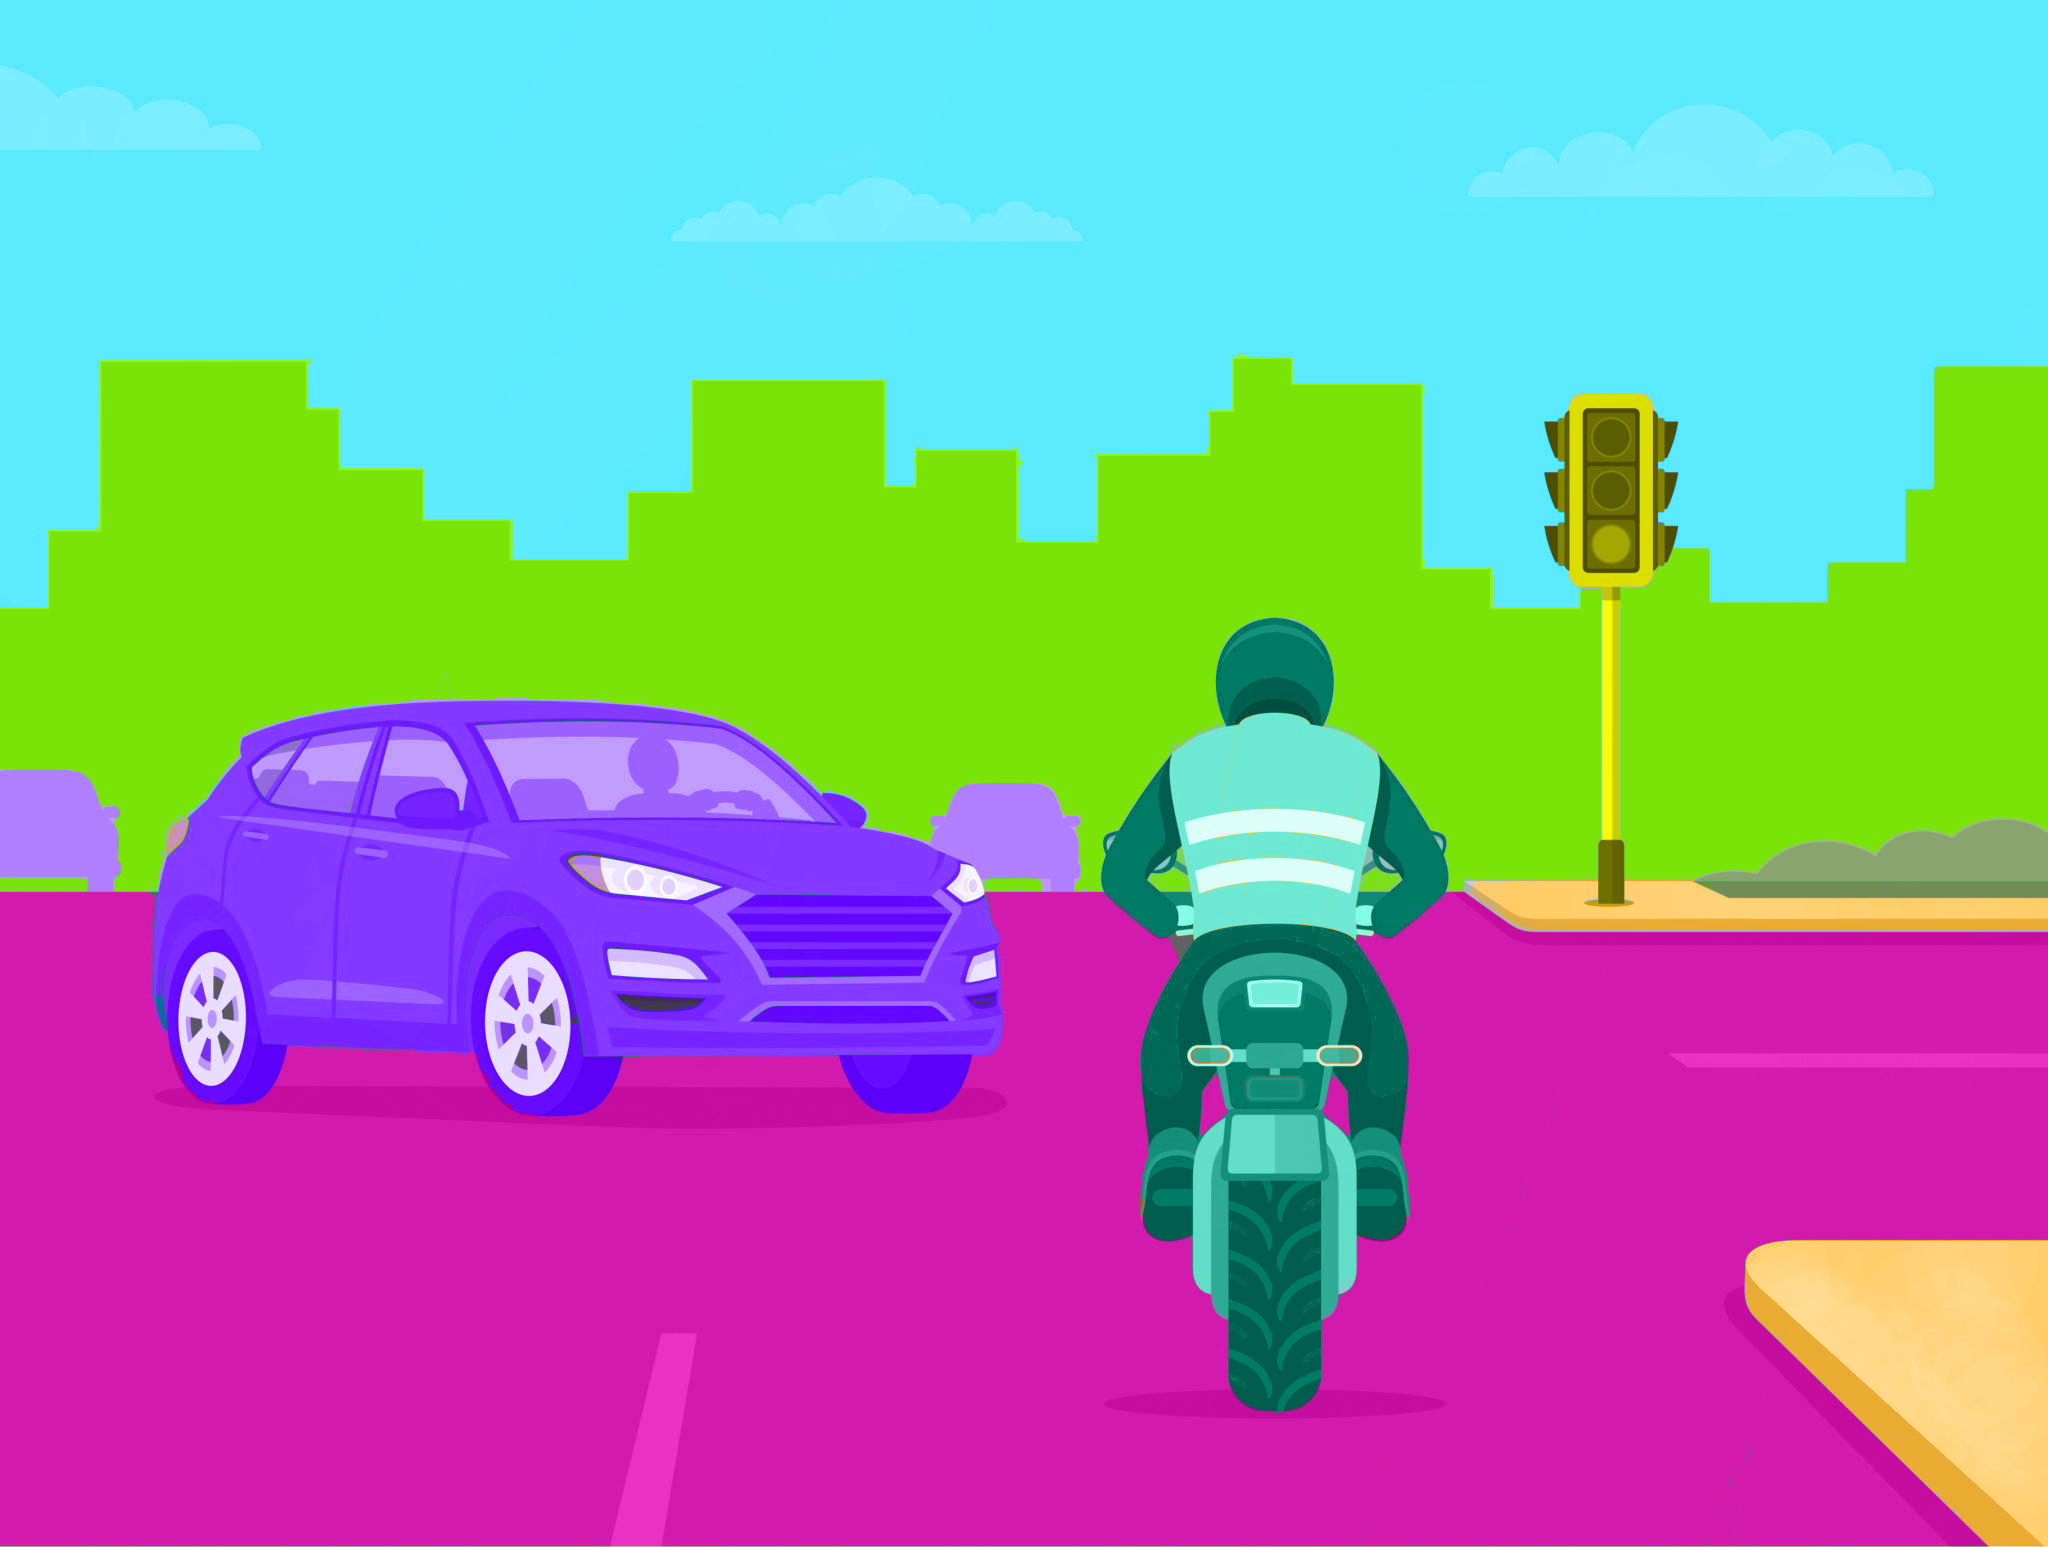
\includegraphics[width=0.9\textwidth]{resources/images/semantic_segmentation.png}
            \captionsetup{labelformat=empty}
            \caption{Semântica}
        \end{figure}
        % {\Huge\setstretch{1.0} Semântica\par}

      \column{0.4\textwidth}
        \begin{figure}[h]
            \centering
            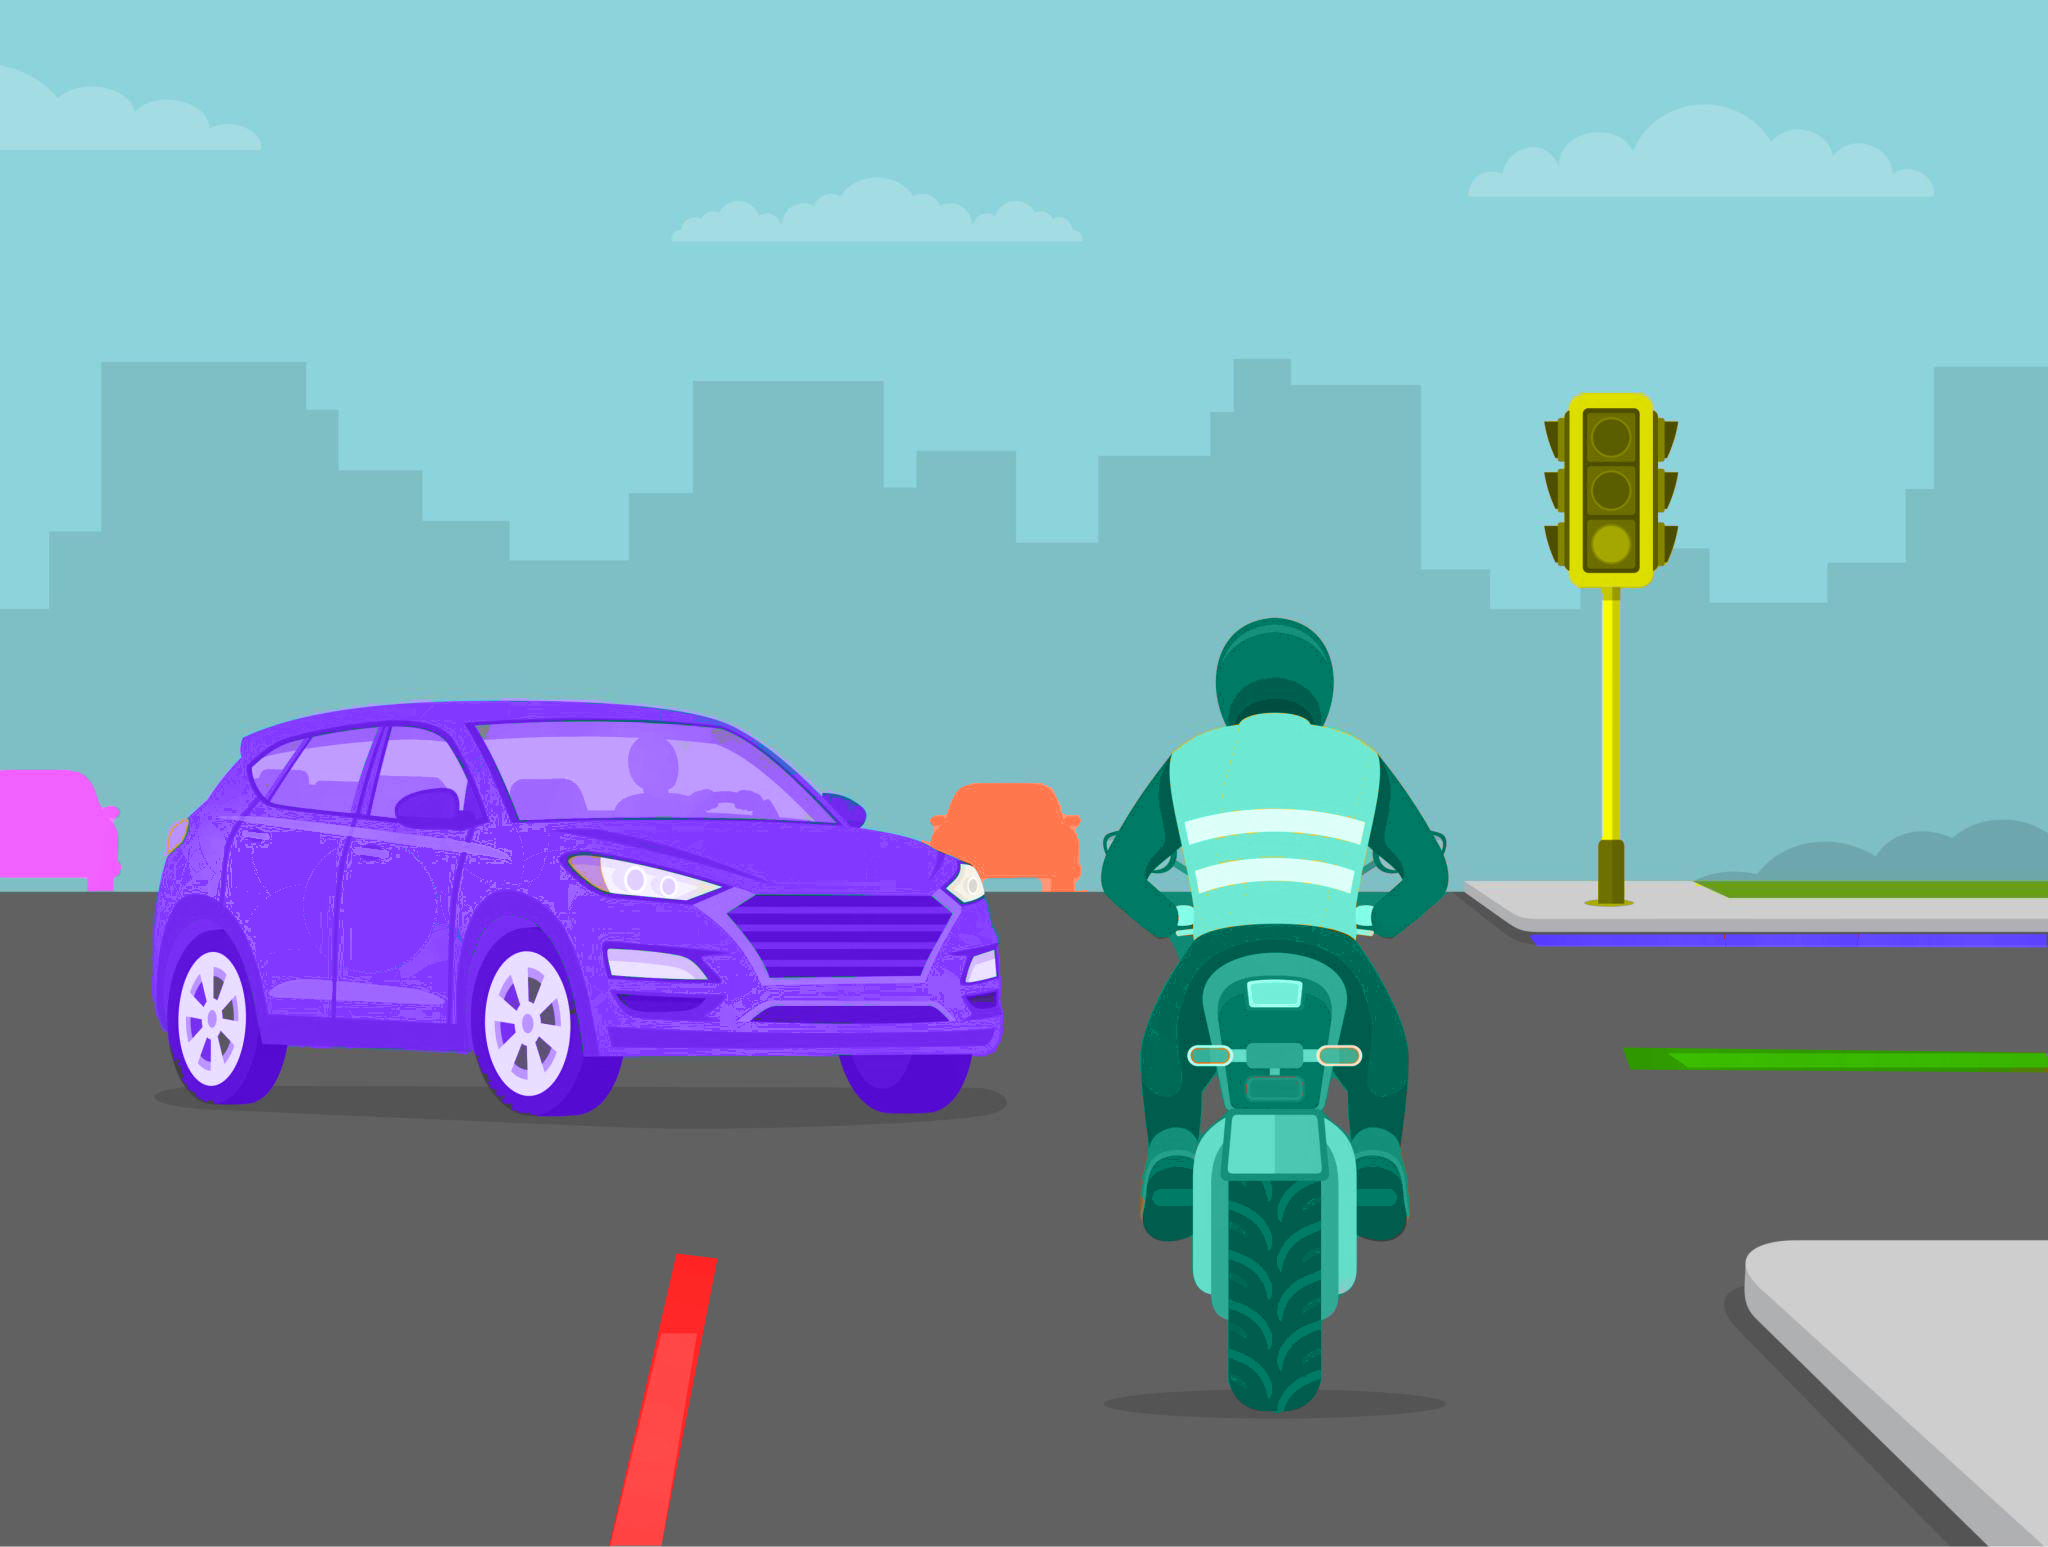
\includegraphics[width=0.9\textwidth]{resources/images/instance_segmentation.png}
            \captionsetup{labelformat=empty}
            \caption{De instâncias}
        \end{figure}
    \end{columns}
        \vspace{\fill}
        \vspace{-0.2cm}


      % {\Huge\centering\setstretch{1.0} Panóptica\par}

        \begin{figure}[h]
            \centering
            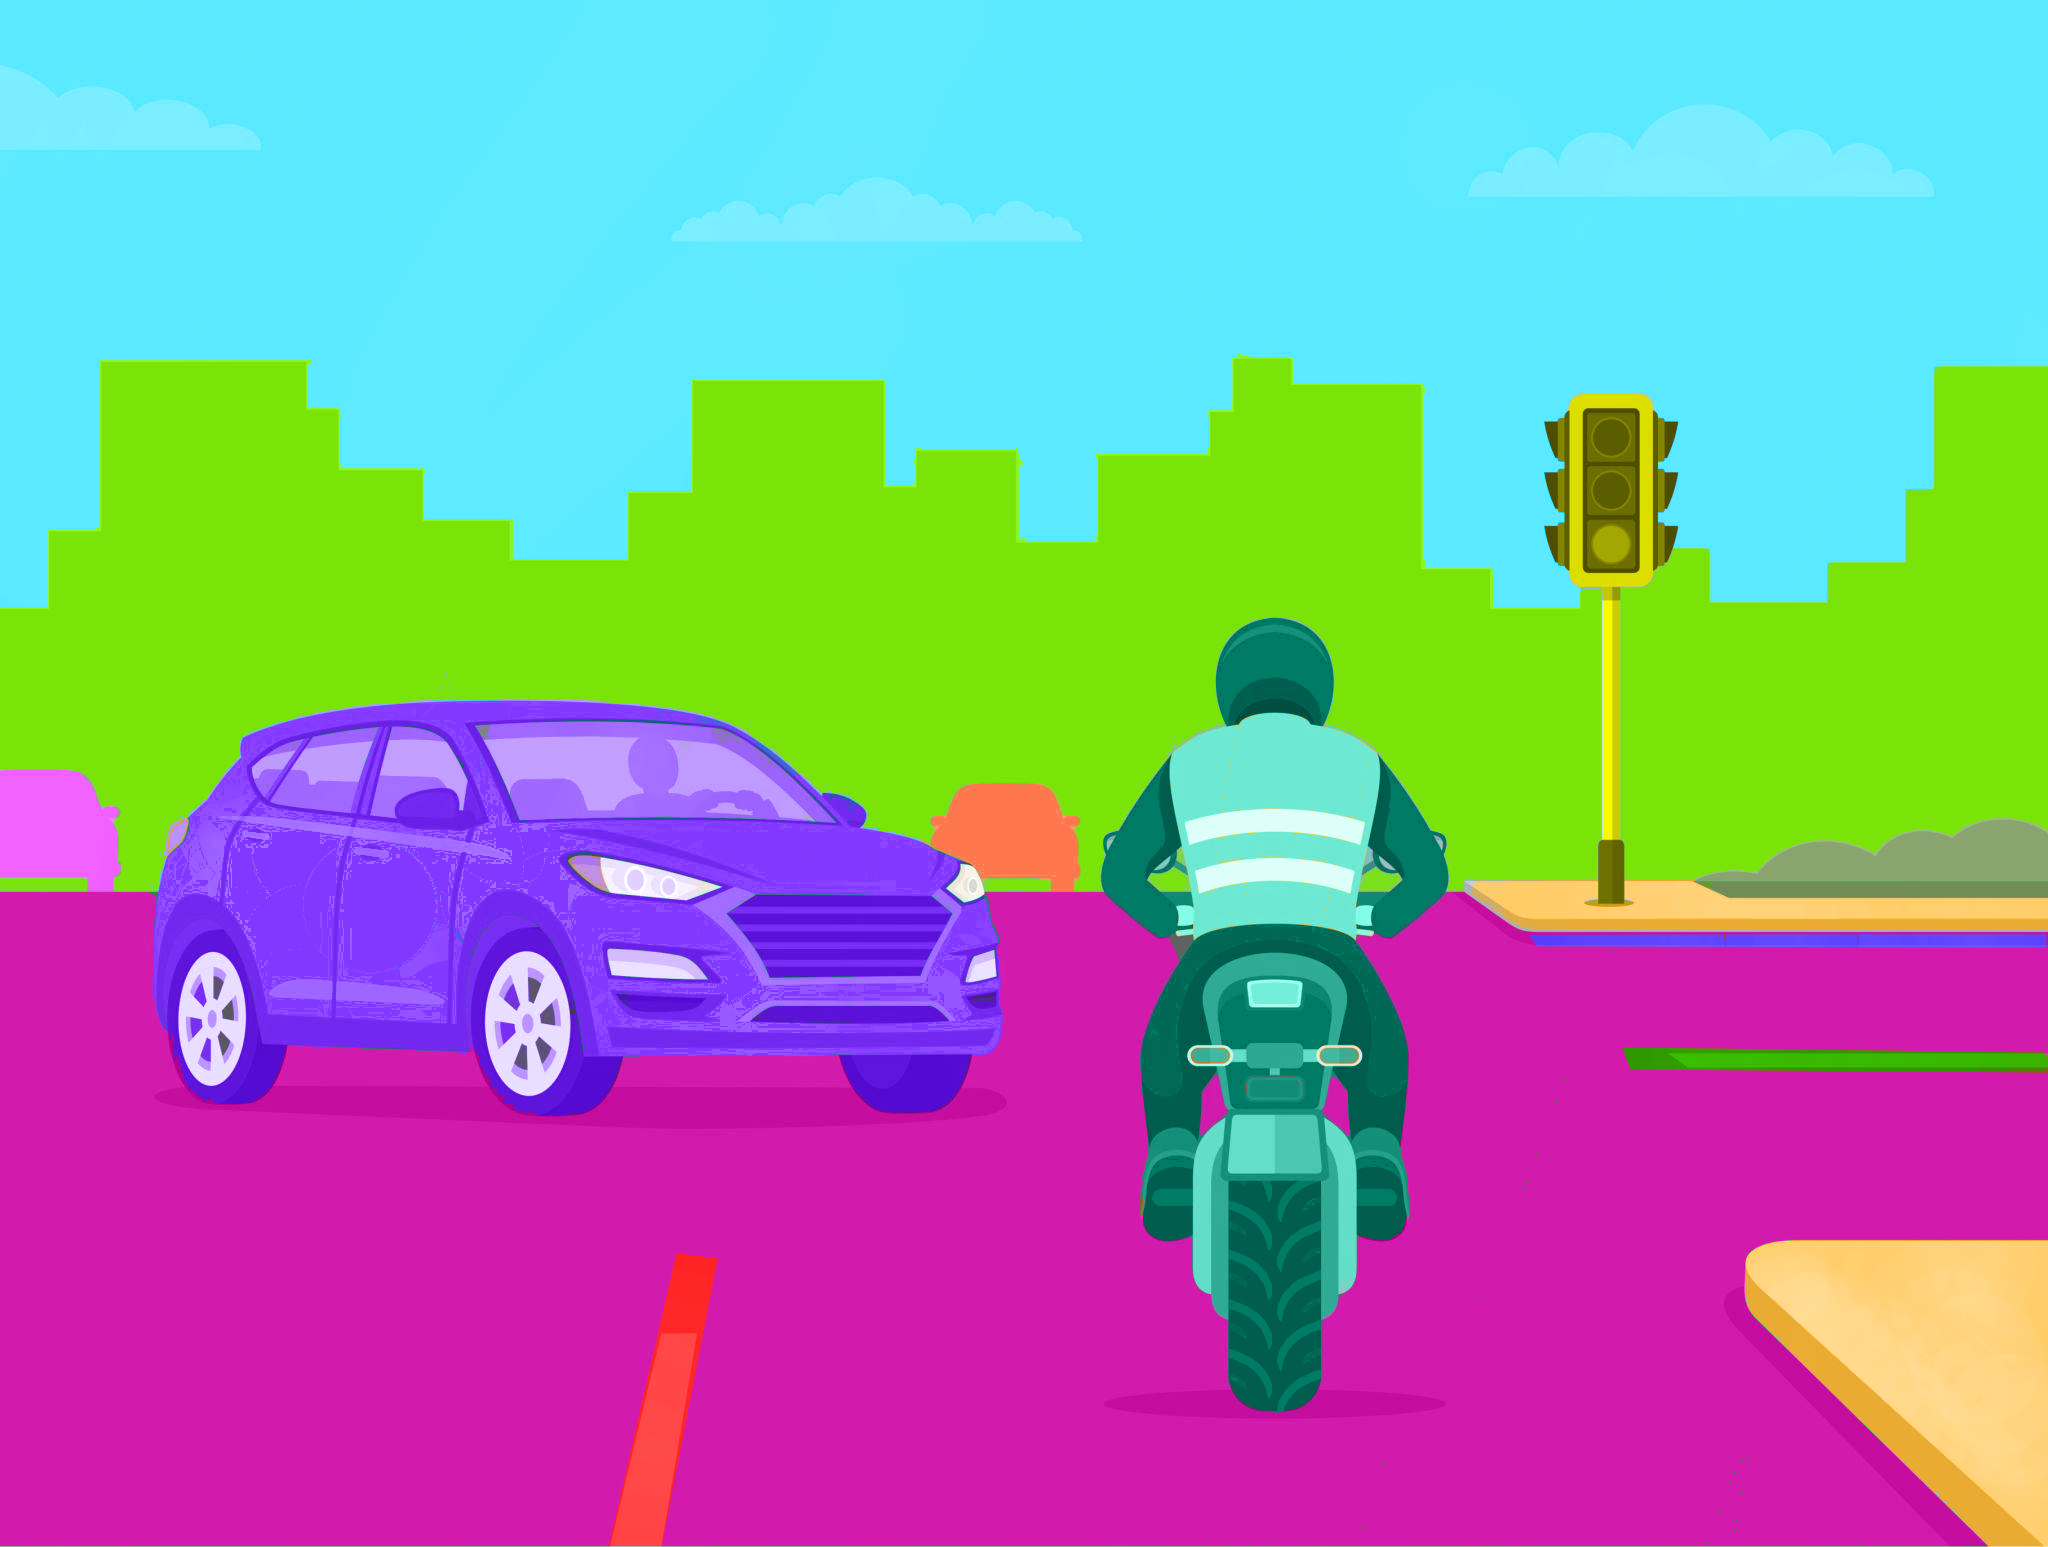
\includegraphics[width=0.36\textwidth]{resources/images/panoptic_segmentation.png}
            \captionsetup{labelformat=empty}
            \caption{Panóptica}
        \end{figure}

\end{frame}
